\newpage

\section{Sprint Backlogs}

In Figures~\ref{fig:sprint_1}~-~\ref{fig:sprint_4}, the issue backlog can
be found. The list for each sprint consists of the issues that were planned
for that particular sprint. A green background implies that the issue was
actually addressed, a red background implies that it had to be postponed to
a later sprint.

\begin{figure}[H]
\centering
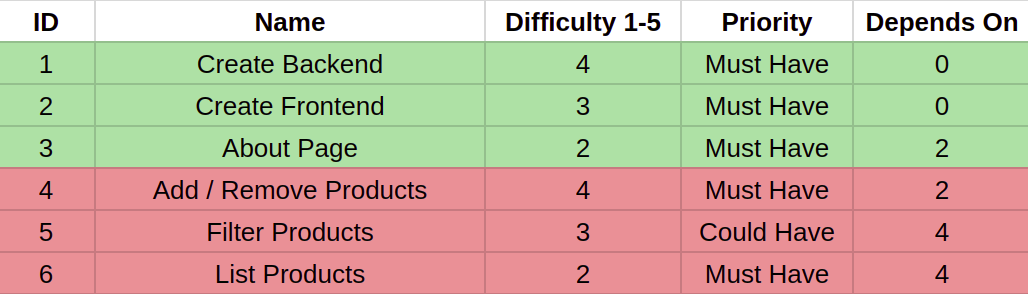
\includegraphics[width=\textwidth]{second_sprint/sprint_1.png}
\caption{\label{fig:sprint_1} Issues, Sprint 1.}
\end{figure}

\begin{figure}[H]
\centering
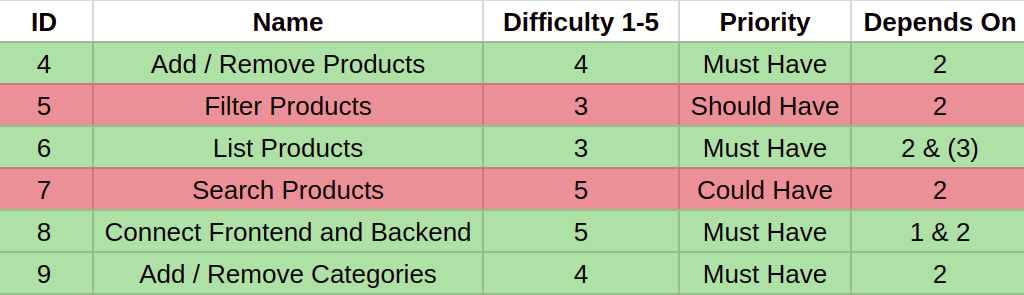
\includegraphics[width=\textwidth]{second_sprint/sprint_2.png}
\caption{\label{fig:sprint_2} Issues, Sprint 2.}
\end{figure}

\begin{figure}[H]
\centering
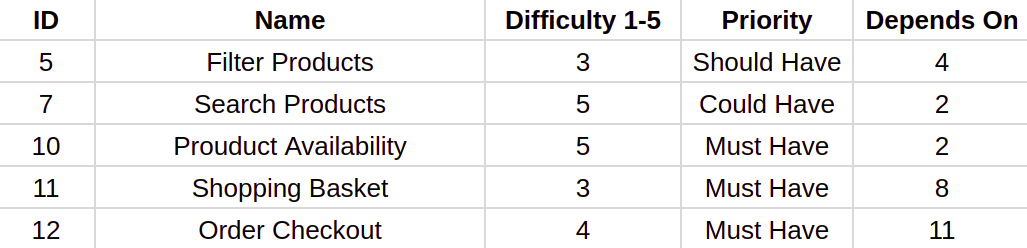
\includegraphics[width=\textwidth]{second_sprint/sprint_3.png}
\caption{\label{fig:sprint_3} Issues, Sprint 3.}
\end{figure}

\begin{figure}[H]
\centering
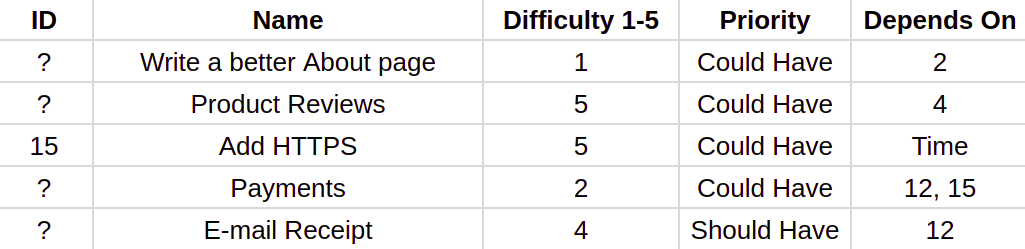
\includegraphics[width=\textwidth]{second_sprint/other.png}
\caption{\label{fig:sprint_4} Issues that have not yet been assigned to
a sprint}
\end{figure}
